\chapter{Run II Preparation}
\label{CHAPTER:RunIIPreparation}

\glsresetall % Resetting all acronyms

%%%%%%%%%%%%%%%%%%%%%%%%%%%%%%%%%%%%%%%%%%%%%%%%%%%%%%%%%%%%%%%%%%%%%%%%%%%%%%%%%%%%%%%
%%% SECTION
%%%%%%%%%%%%%%%%%%%%%%%%%%%%%%%%%%%%%%%%%%%%%%%%%%%%%%%%%%%%%%%%%%%%%%%%%%%%%%%%%%%%%%%
\section{Run II trigger studies}
\label{SECTION:RunIITriggerStudies}

%%%%%%%%%%%%%%%%%%%%%%%%%%%%%%%%%%%%%%%%%%%%%%%%%%%%%%%%%%%%%%%%%%%%%%%%%%%%%%%%%%%%%%%
%%% SECTION
%%%%%%%%%%%%%%%%%%%%%%%%%%%%%%%%%%%%%%%%%%%%%%%%%%%%%%%%%%%%%%%%%%%%%%%%%%%%%%%%%%%%%%%
\section{Run II QCD Monte Carlo samples}
\label{SECTION:RunIIQCDMonteCarloSamples}

Simulating and reconstructing quantities of \gls{QCD} events comparable to the ones produced at the \gls{LHC} experiments is impractical. At every second of \gls{LHC} physics operation several millions of bunch crossings happen, each one able to provoke several simultaneous collisions. With the currently available hardware it takes in excess of one minute to fully simulate one of such bunch crossings. 


This constraints lead to \gls{QCD} events being simulated in $p_\perp$ hats, where the first collision is generated within range where the outgoing particles summed $p_\perp$ is in a predefined range. Then several other collisions are added to the event as \gls{PU}. This additional collisions are generated without any constraints in $p_\perp$. 

This bin method allows the user to have samples with increasing energy and study the influence of each of them in their own analysis. As a practical example we do not need to look over millions of \gls{QCD} events, most of them with only low energy particles, to find high energy jets. We can just start from the higher \gls{QCD} $p_\perp$ hats add lower ones until the stop contributing to our selection. On the other hand, there are some analysis that require jets and/or \gls{MET} with very low values where inclusive \gls{QCD} samples will not have enough statistics to provide insight into the \gls{QCD} behaviour. The \gls{CMS} \gls{VBF} Higgs to invisible analysis is one of them.

During the preparation of the Run I \gls{VBF} Higgs to invisible analysis a set of \gls{QCD} samples with \gls{VBF} like jets and real \gls{MET} was generated. This samples allowed to understand the mechanisms that create real \gls{MET} in \gls{QCD} and how those could be mitigated.

Our analysis is now preparing for Run II it was considered once again to be useful to have similar samples remade and possibly extended. It was identified that not only real \gls{MET} is significant but also fake \gls{MET} coming from detector miss-measurement. If such a sample could be produced and simulate such effects would be of great interest, allowing the analysis to possibly evolve to a shape based analysis or event to use machine learning techniques.

This study investigates the alternatives and attempts to quantify the costs of of producing such samples.








% Total number of events: 17871
% 
% => Event counters:
% Jet Matched not lowest DeltaR : 1866
% Selected diparton has a match : 13218
% 
% pt>30 : 687 : 14 : 0.0203785 
% 
% pt>30 : 1467 : 49 : 0.0334015   

%%%%%%%%%%%%%%%%%%%%%%%%%%%%%%%%%%%%%%%%%%%%%%%%%%%%%%%%%%%%%%%%%%%%%%%%%%%%%%%%%%%%%%%
%%% SUBSECTION
%%%%%%%%%%%%%%%%%%%%%%%%%%%%%%%%%%%%%%%%%%%%%%%%%%%%%%%%%%%%%%%%%%%%%%%%%%%%%%%%%%%%%%%
\subsection{Gridpack Validation}
\label{SUBSECTION:GridpackValidation}

\begin{table}
\centering

\resizebox{1.0\textwidth}{!}{
\begin{tabular}{|c|c|c|c|c|c|}
\hline
                          & \multicolumn{3}{c|}{Events}      & \multicolumn{2}{c|}{Cross Section [pb]}                                       \\
\hline
Process                   & Tried  & Passed & accepted [\%]  & Before                                & After                                 \\
\hline\hline 
$p p \rightarrow j j$     &  30295 &   7252 & $23.9 \pm 0.2$ & $1.673e+06 \pm 8.616e+03$ & $4.005e+05 \pm 4.591e+03$ \\
$p p \rightarrow j j j$   &  64985 &   4776 & $ 7.3 \pm 0.1$ & $3.547e+06 \pm 1.826e+04$ & $2.607e+05 \pm 3.871e+03$ \\
$p p \rightarrow j j j j$ &  89720 &   5843 & $ 6.5 \pm 0.1$ & $4.939e+06 \pm 2.543e+04$ & $3.216e+05 \pm 4.393e+03$ \\
\hline\hline
Total                     & 185000 &  17871 & $ 9.7 \pm 0.1$ & $1.016e+07 \pm 3.247e+04$ & $9.828e+05 \pm 7.440e+03$ \\
\hline
\end{tabular}
}
\caption{TODO:}

\end{table}




% --------------------------------------------------------------------------------------------------------------------------------------------------------------------------                                                                                                    
% Overall cross-section summary                                                                                                                                                                                                                                                 
% --------------------------------------------------------------------------------------------------------------------------------------------------------------------------                                                                                                    
% Process         xsec_before [pb]                passed  nposw   nnegw   tried   nposw   nnegw   xsec_match [pb]                 accepted [%]     event_eff [%]                                                                                                                
% 0               1.673e+06 +/- 8.616e+03         7252    7252    0       30295   30295   0       4.005e+05 +/- 4.591e+03         23.9 +/- 0.2    23.9 +/- 0.2                                                                                                                  
% 1               3.547e+06 +/- 1.826e+04         4776    4776    0       64985   64985   0       2.607e+05 +/- 3.871e+03         7.3 +/- 0.1     7.3 +/- 0.1                                                                                                                   
% 2               4.939e+06 +/- 2.543e+04         5843    5843    0       89720   89720   0       3.216e+05 +/- 4.393e+03         6.5 +/- 0.1     6.5 +/- 0.1                                                                                                                   
% --------------------------------------------------------------------------------------------------------------------------------------------------------------------------                                                                                                    
% Total           1.016e+07 +/- 3.247e+04         17871   17871   0       185000  185000  0       9.828e+05 +/- 7.440e+03         9.7 +/- 0.1     9.7 +/- 0.1
% --------------------------------------------------------------------------------------------------------------------------------------------------------------------------
% Before matching: total cross section = 1.016e+07 +- 3.247e+04 pb
% After matching: total cross section = 9.828e+05 +- 7.440e+03 pb
% Filter efficiency (taking into account weights)= (17871) / (17871) = 1.000e+00 +- 0.000e+00
% Filter efficiency (event-level)= (17871) / (17871) = 1.000e+00 +- 0.000e+00
% After filter: final cross section = 9.828e+05 +- 7.440e+03 pb


\begin{table}[!htp]
\centering

\begin{tabular}{|c||c|c|c||c|}
\hline
            &          \multicolumn{4}{c|}{Process} \\
\hline
$n_{match}$ &      jj &    jjj  &    jjjj &   Total \\
\hline\hline 
          0 & 03.54\% &  0.29\% & 00.05\% & 01.53\% \\
          1 & 25.21\% &  4.23\% & 01.35\% & 11.80\% \\
          2 & 71.25\% & 27.55\% & 08.66\% & 39.11\% \\
          3 &         & 67.92\% & 36.16\% & 29.98\% \\
          4 &         &         & 53.77\% & 17.58\% \\
\hline
\end{tabular}
\caption{TODO:}

\end{table}

% => Parton to GenJet matching results:
% all partons entries 17871
% Matched #0 partons:  274 fraction: 0.0153321
% Matched #1 partons: 2109 fraction: 0.118012
% Matched #2 partons: 6989 fraction: 0.391081
% Matched #3 partons: 5357 fraction: 0.299759
% Matched #4 partons: 3142 fraction: 0.175816
% 
% jj partons entries 7252
% Matched #0 partons:  257 fraction: 0.0354385
% Matched #1 partons: 1828 fraction: 0.252068
% Matched #2 partons: 5167 fraction: 0.712493
% 
% jjj partons entries 4776
% Matched #0 partons:   14 fraction: 0.00293132
% Matched #1 partons:  202 fraction: 0.0422948
% Matched #2 partons: 1316 fraction: 0.275544
% Matched #3 partons: 3244 fraction: 0.679229
% 
% jjjj partons entries 5843
% Matched #0 partons:    3 fraction: 0.000513435
% Matched #1 partons:   79 fraction: 0.0135205
% Matched #2 partons:  506 fraction: 0.0865993
% Matched #3 partons: 2113 fraction: 0.361629
% Matched #4 partons: 3142 fraction: 0.537737


\begin{figure}[htp]%
\centering
\subfloat[][]{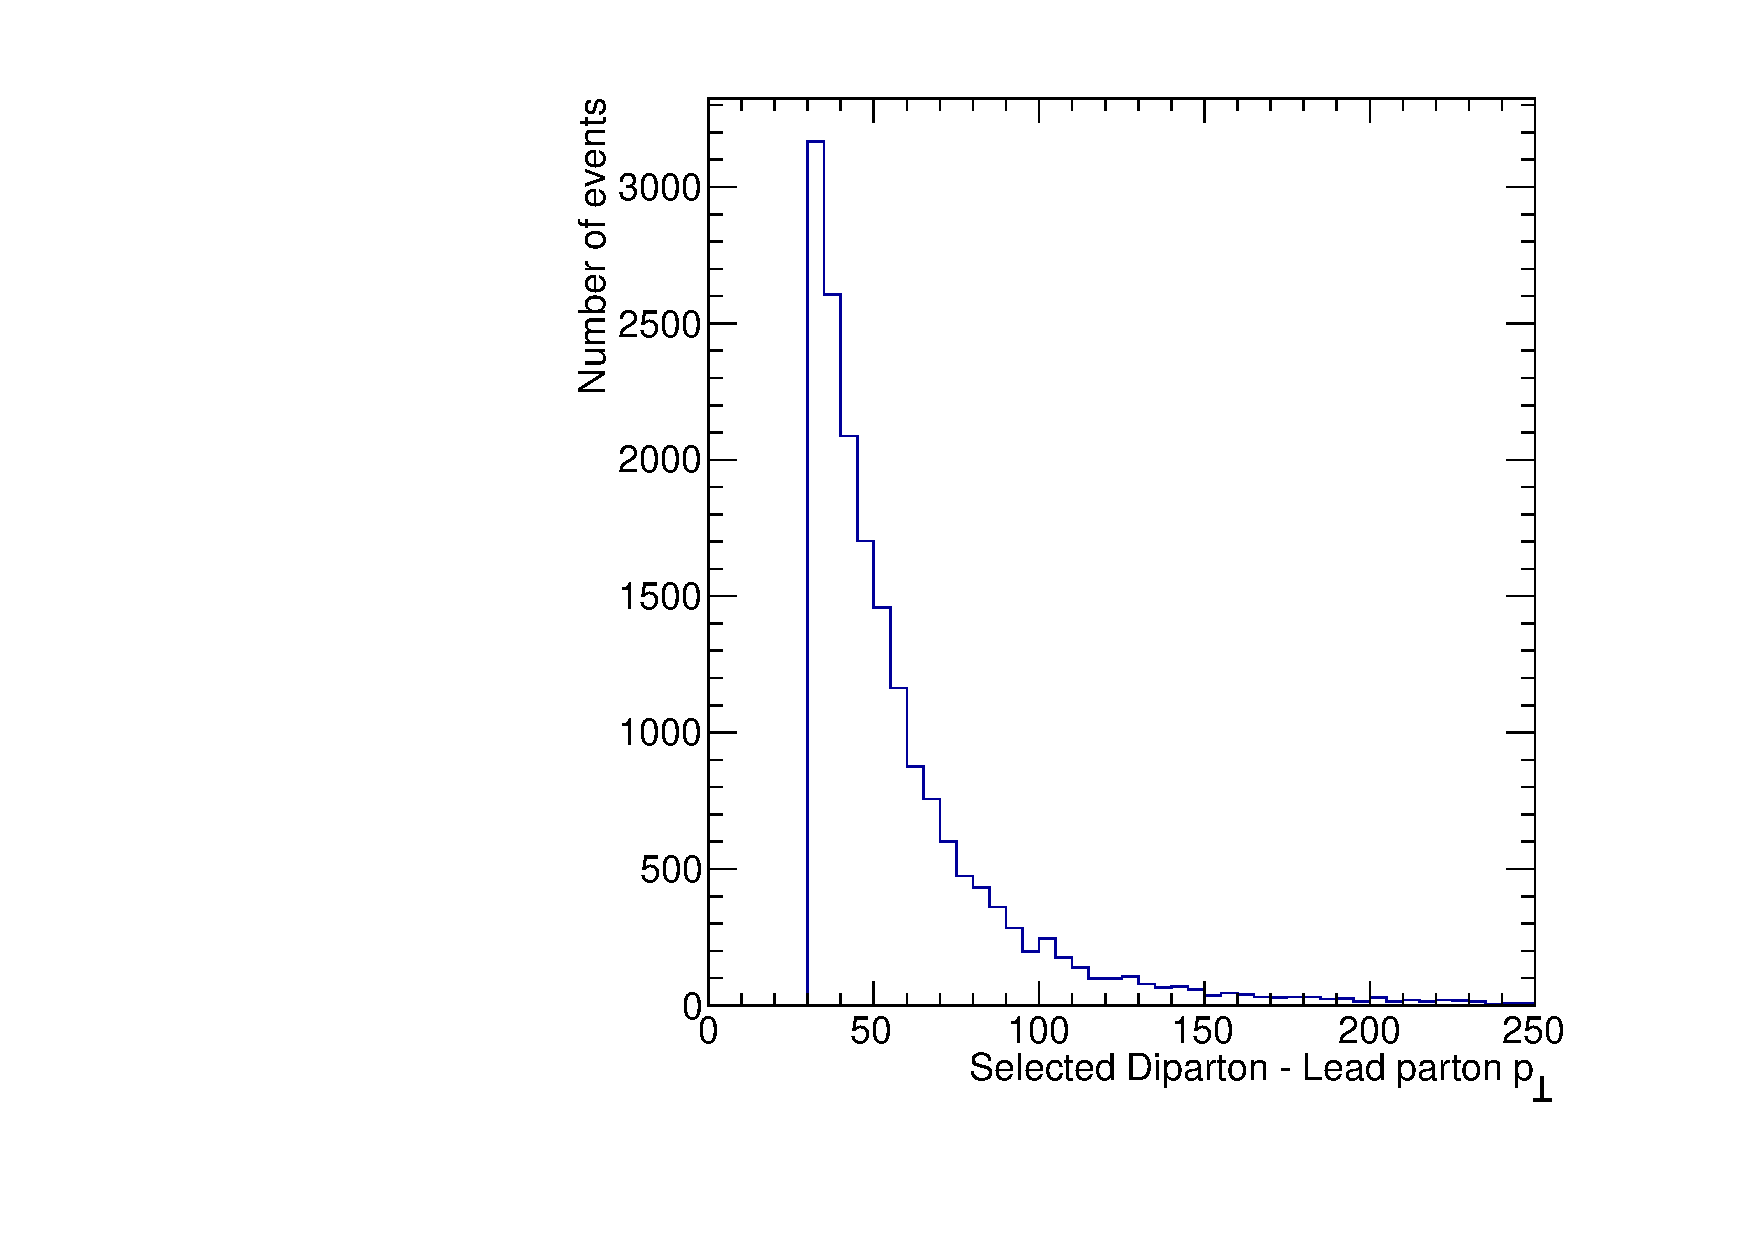
\includegraphics[width=0.45\linewidth]{Chapter07/QCDVBF/Gridpack/Images/SelDiParton_Parton1_Pt.pdf}}\qquad
\subfloat[][]{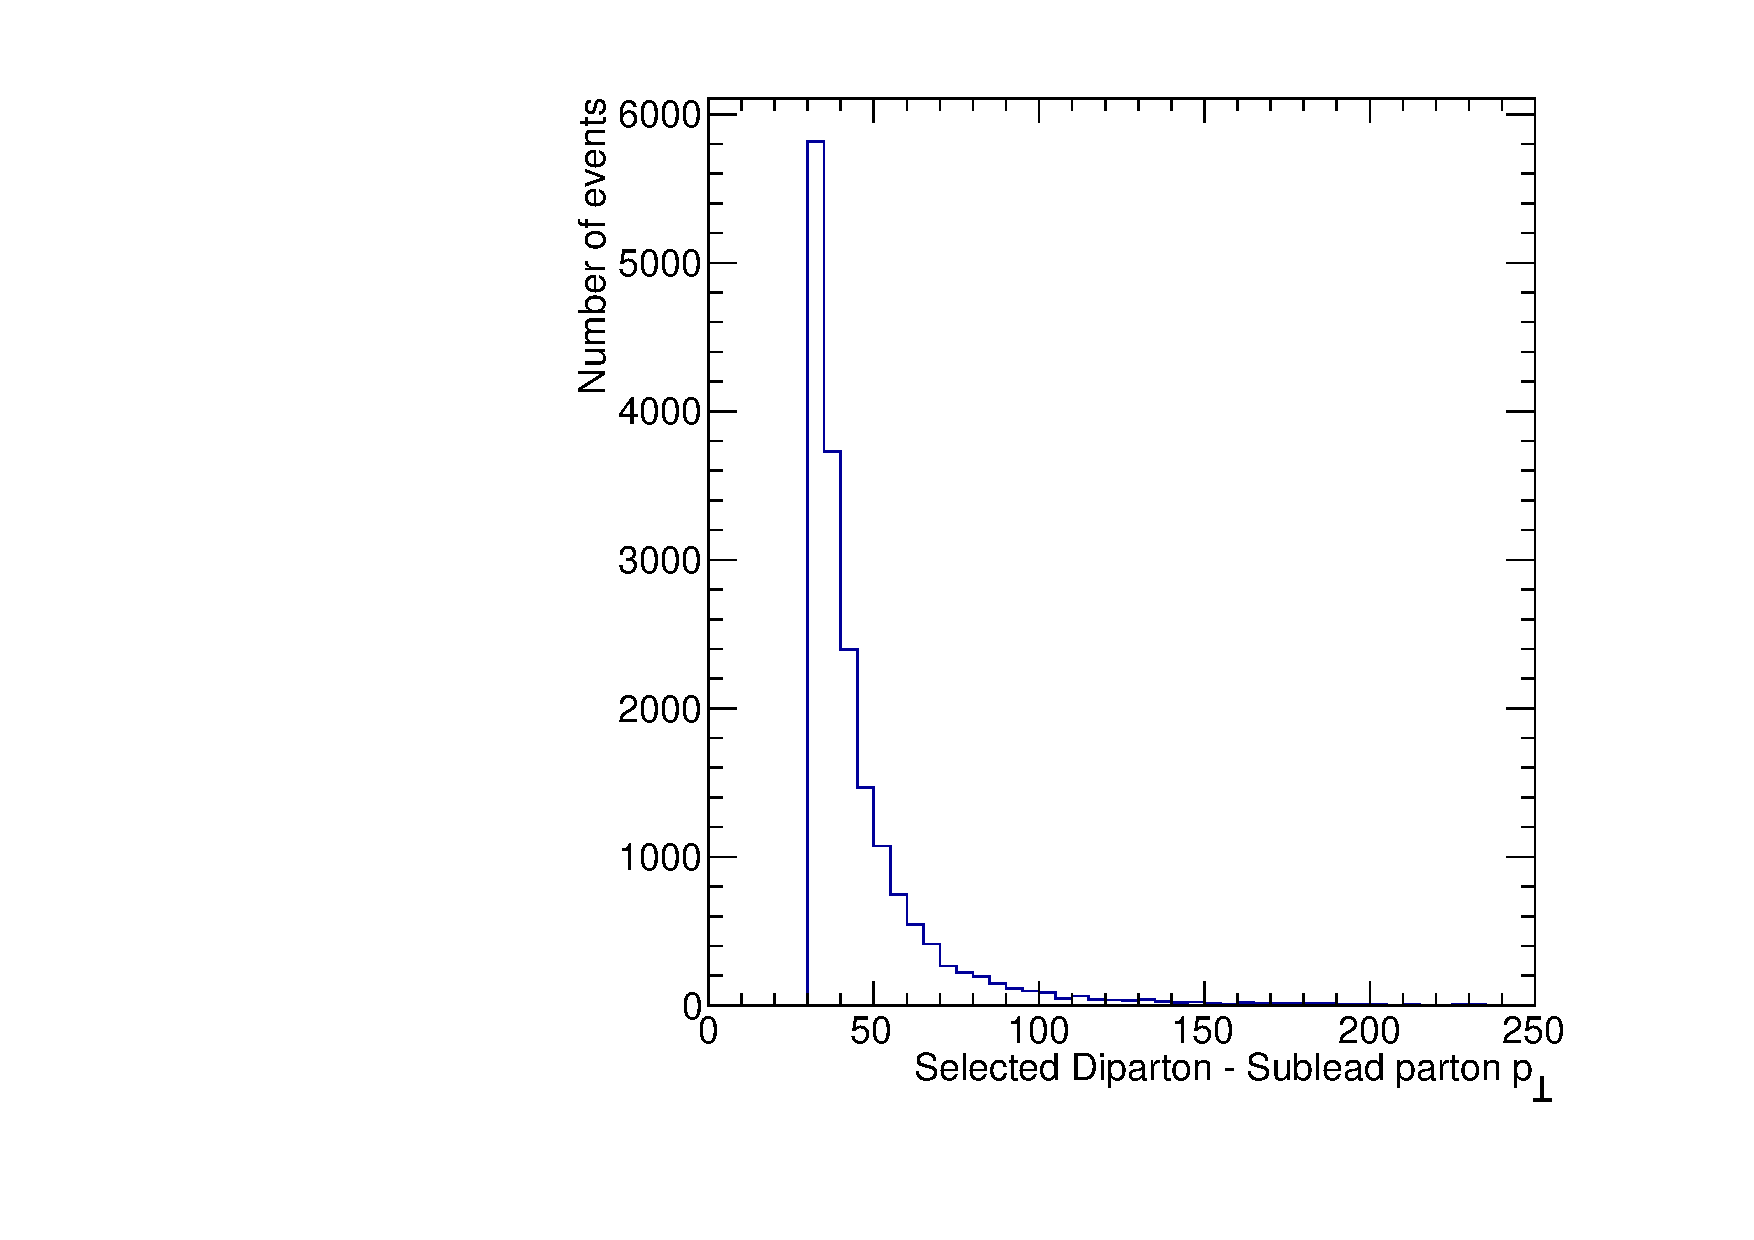
\includegraphics[width=0.45\linewidth]{Chapter07/QCDVBF/Gridpack/Images/SelDiParton_Parton2_Pt.pdf}}\\
\caption[TODO]{TODO}
\label{FIGURE:TODO}
\end{figure}

\begin{figure}[htp]%
\centering
\subfloat[][]{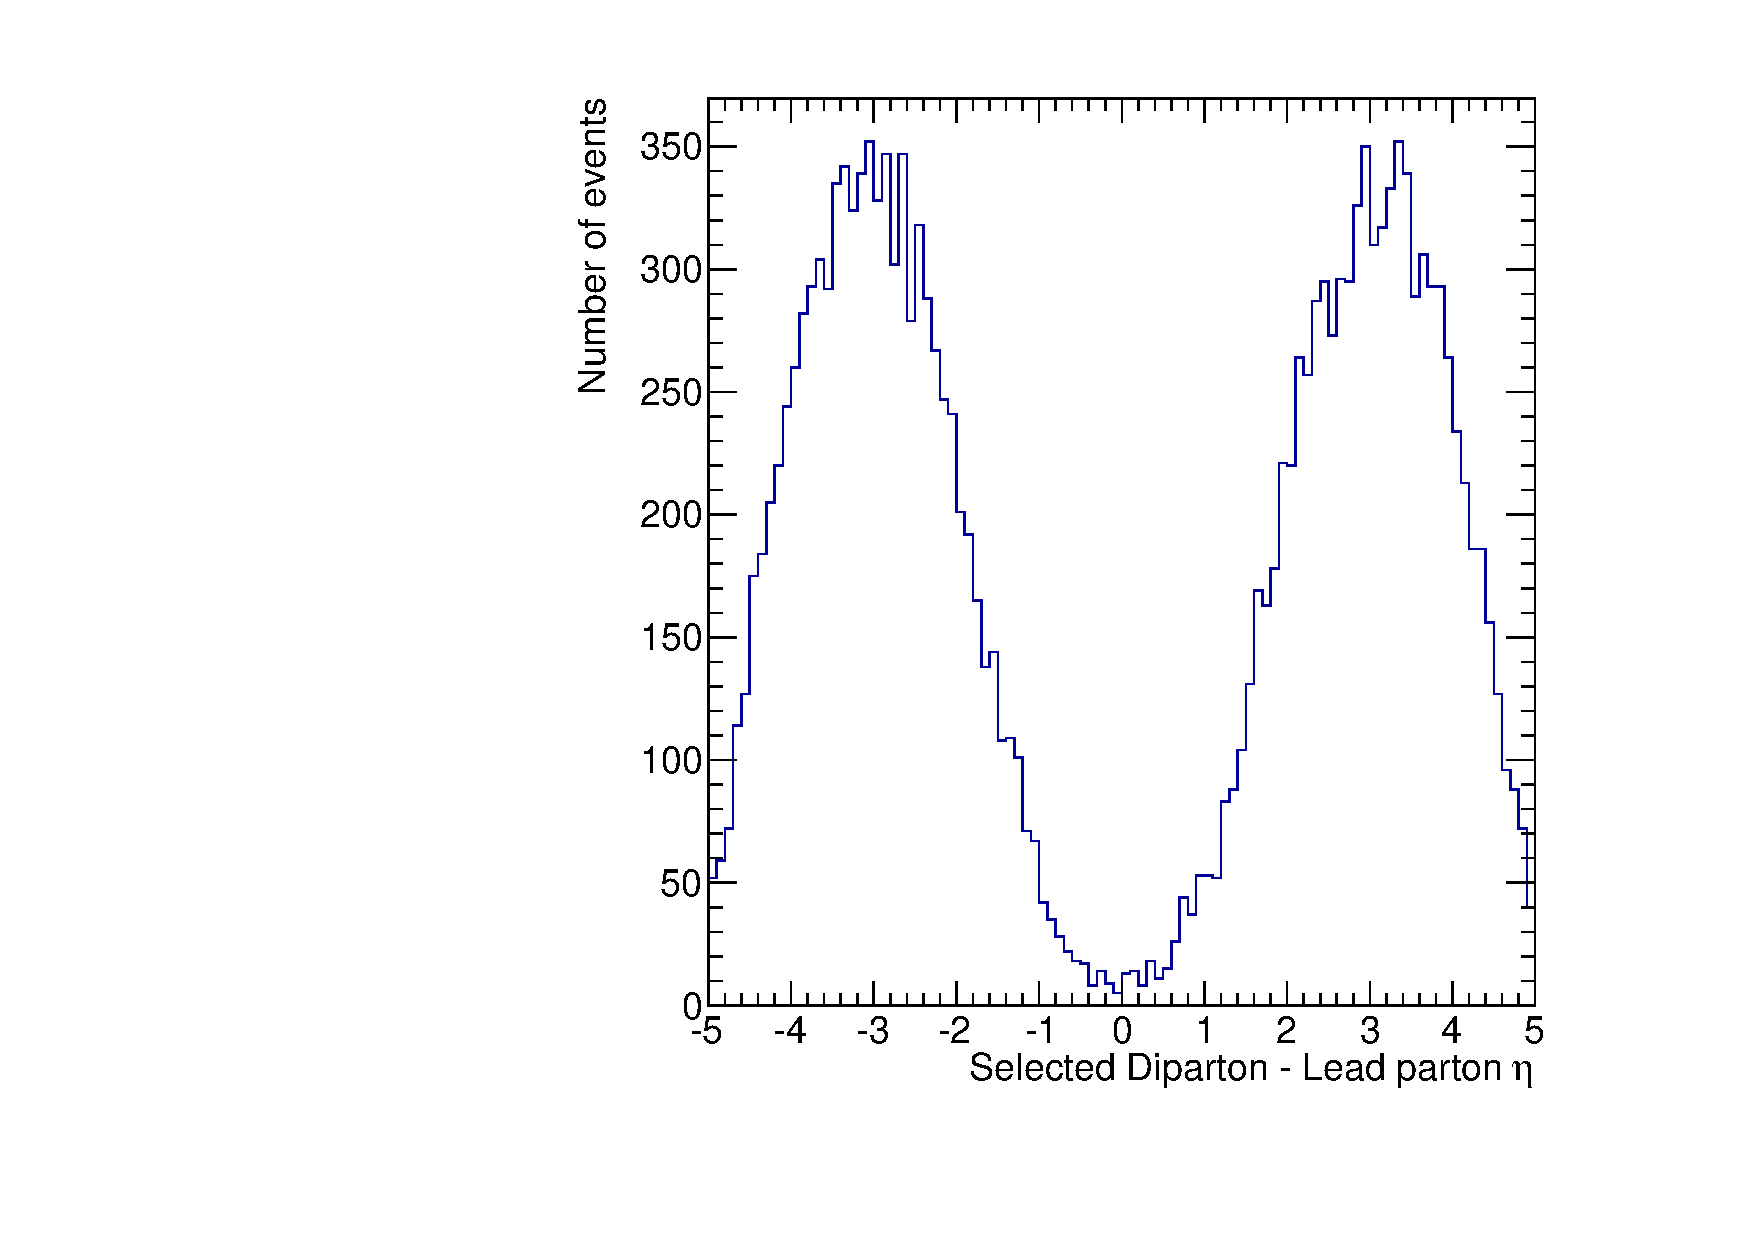
\includegraphics[width=0.45\linewidth]{Chapter07/QCDVBF/Gridpack/Images/SelDiParton_Parton1_Eta.pdf}}\qquad
\subfloat[][]{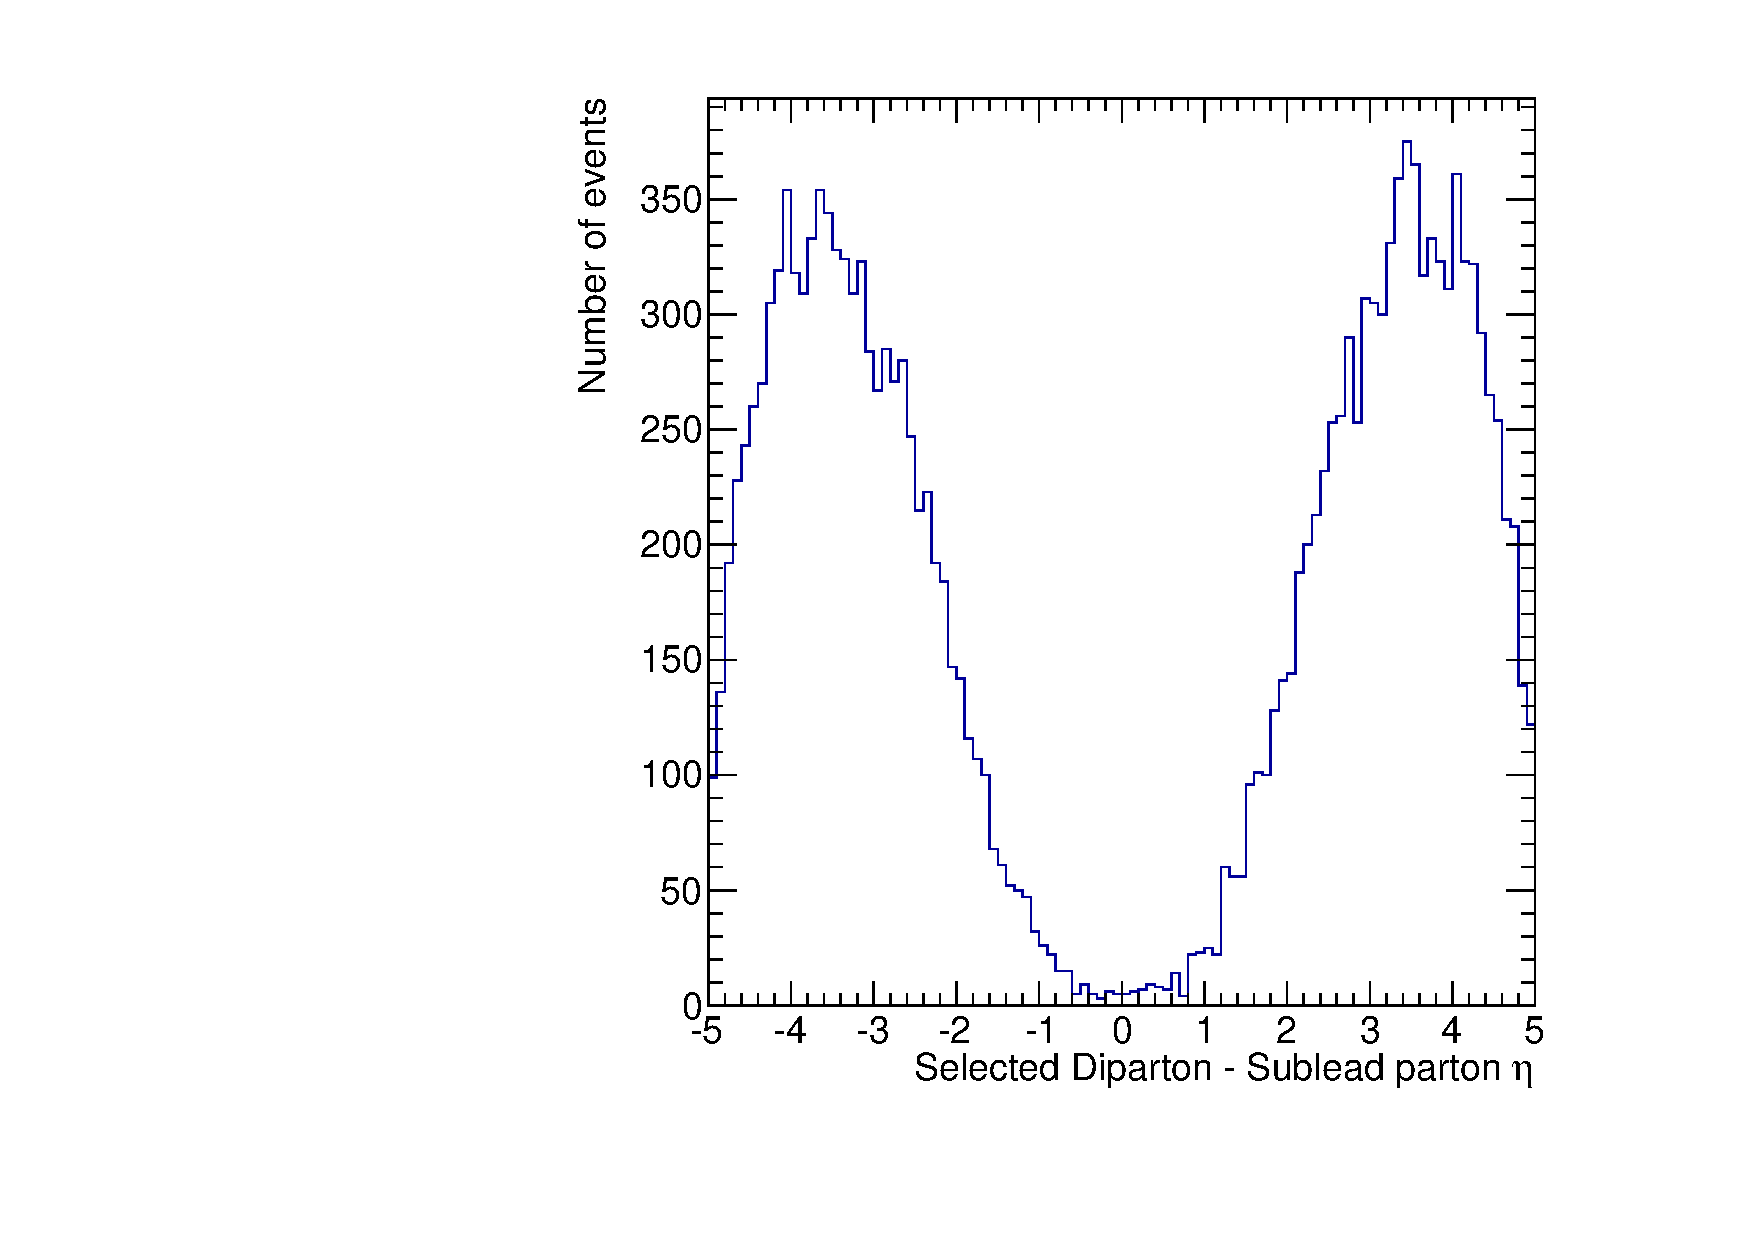
\includegraphics[width=0.45\linewidth]{Chapter07/QCDVBF/Gridpack/Images/SelDiParton_Parton2_Eta.pdf}}\\
\caption[TODO]{TODO}
\label{FIGURE:TODO}
\end{figure}

\begin{figure}[htp]%
\centering
\subfloat[][]{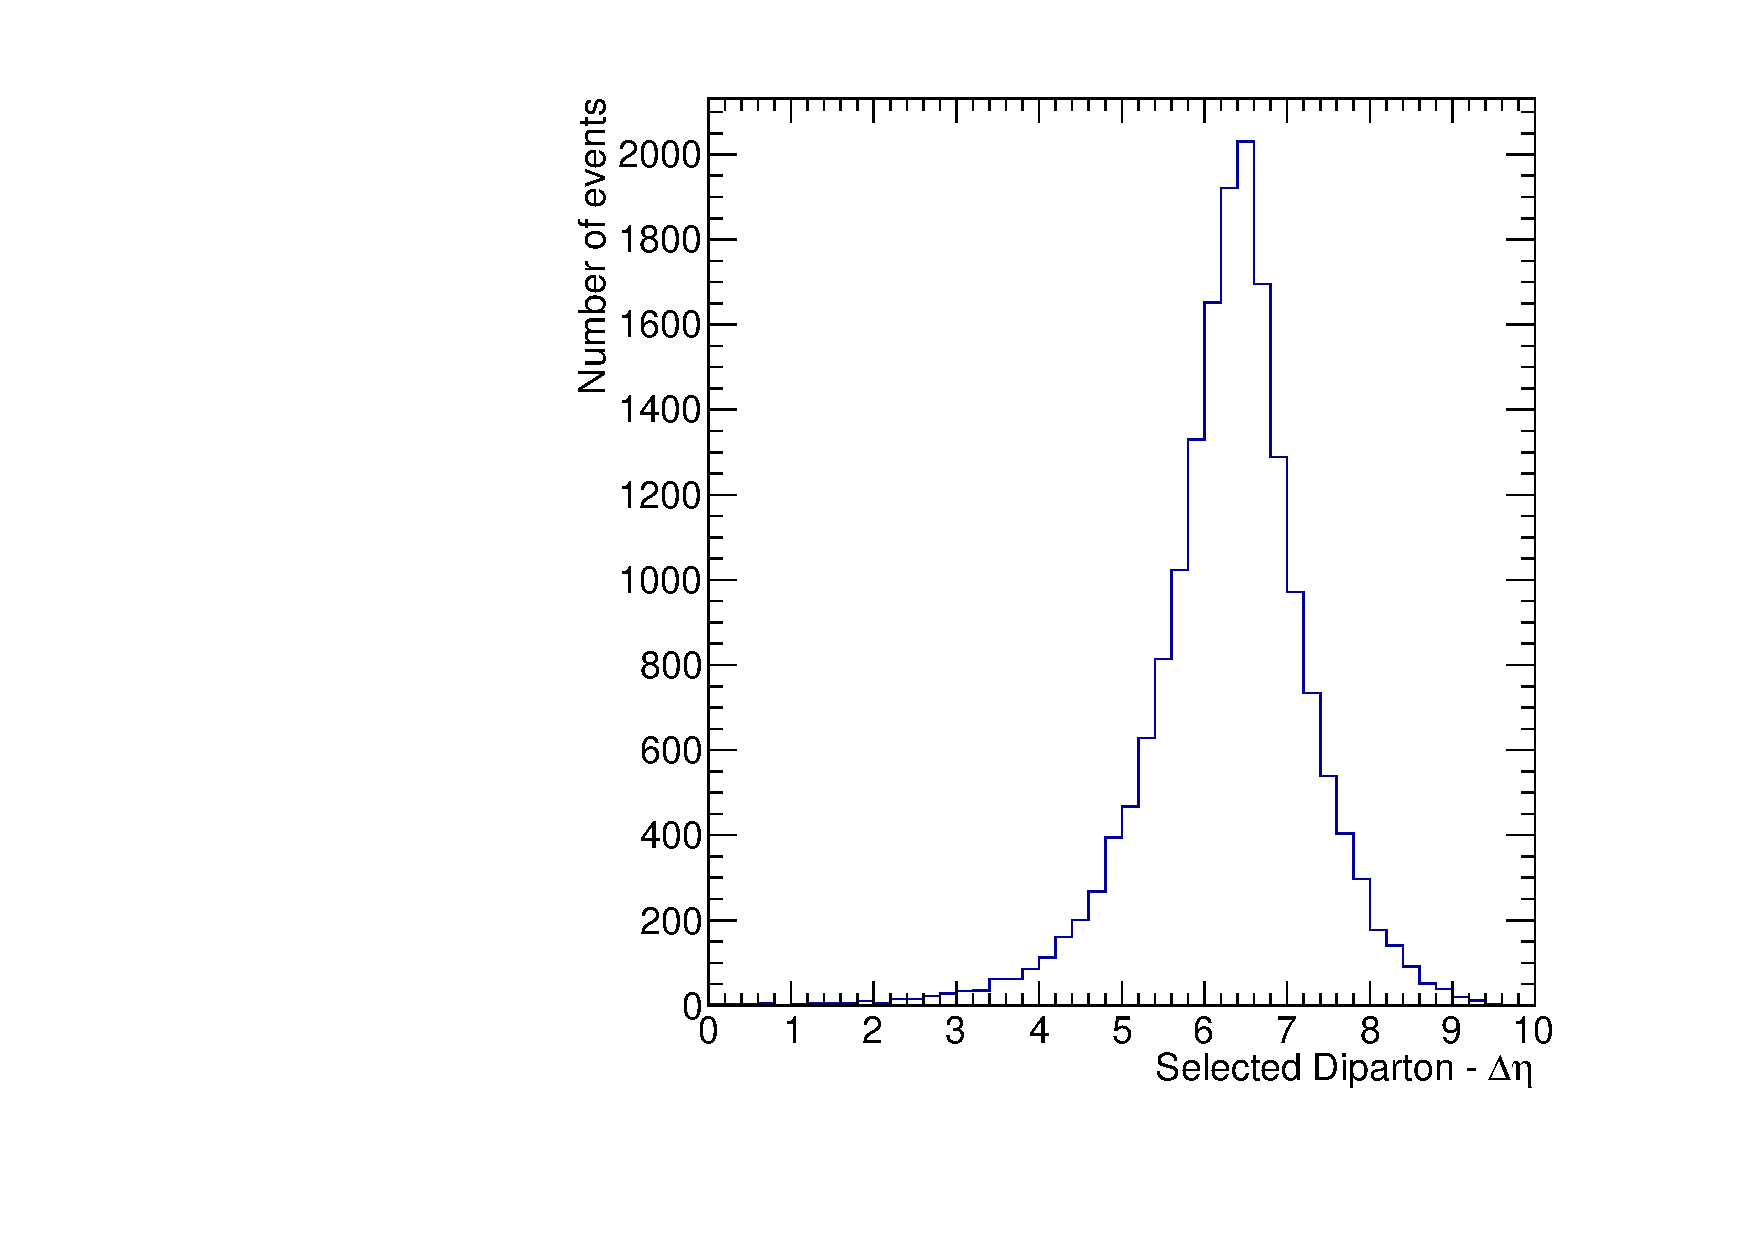
\includegraphics[width=0.45\linewidth]{Chapter07/QCDVBF/Gridpack/Images/SelDiParton_DEta.pdf}}\qquad
\subfloat[][]{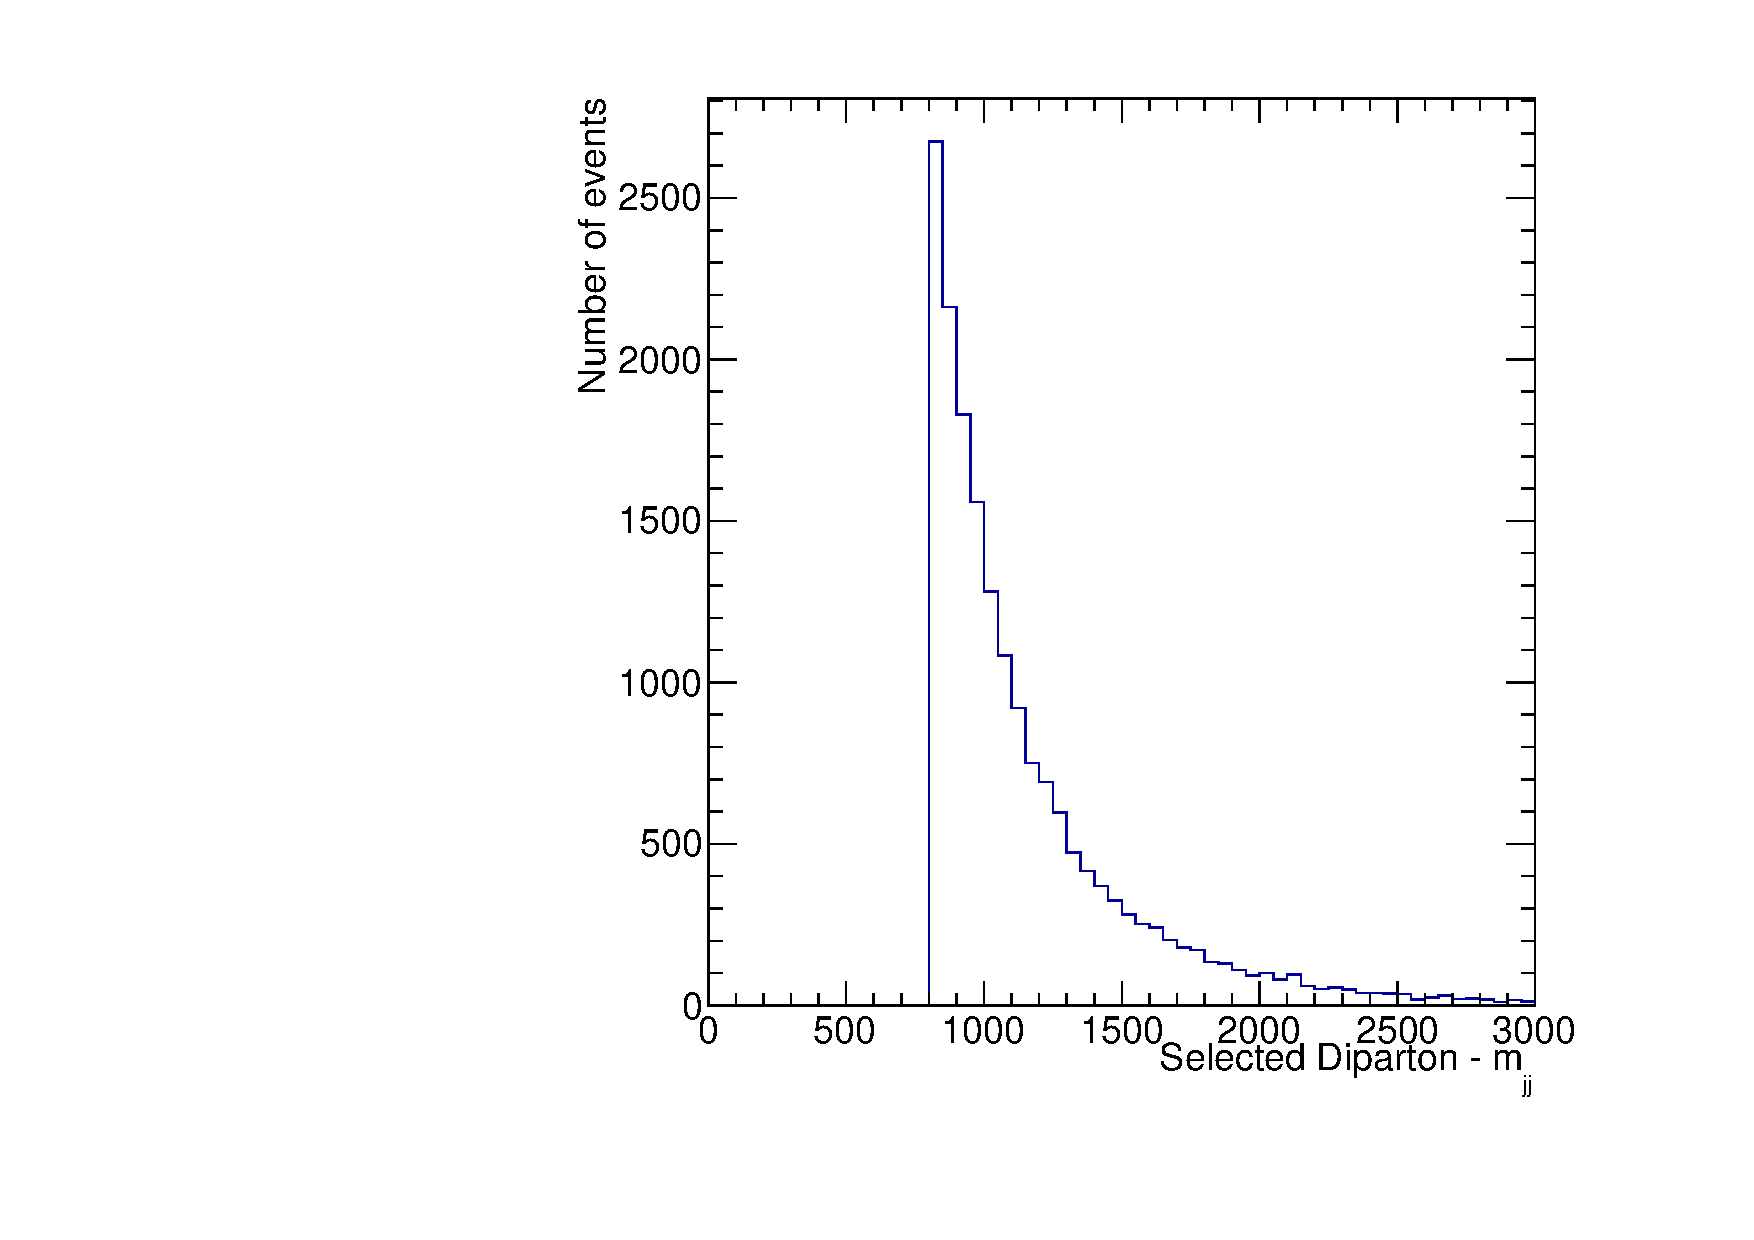
\includegraphics[width=0.45\linewidth]{Chapter07/QCDVBF/Gridpack/Images/SelDiParton_Mjj.pdf}}\\
\caption[TODO]{TODO}
\label{FIGURE:TODO}
\end{figure}

\begin{figure}[htp]%
\centering
\subfloat[][]{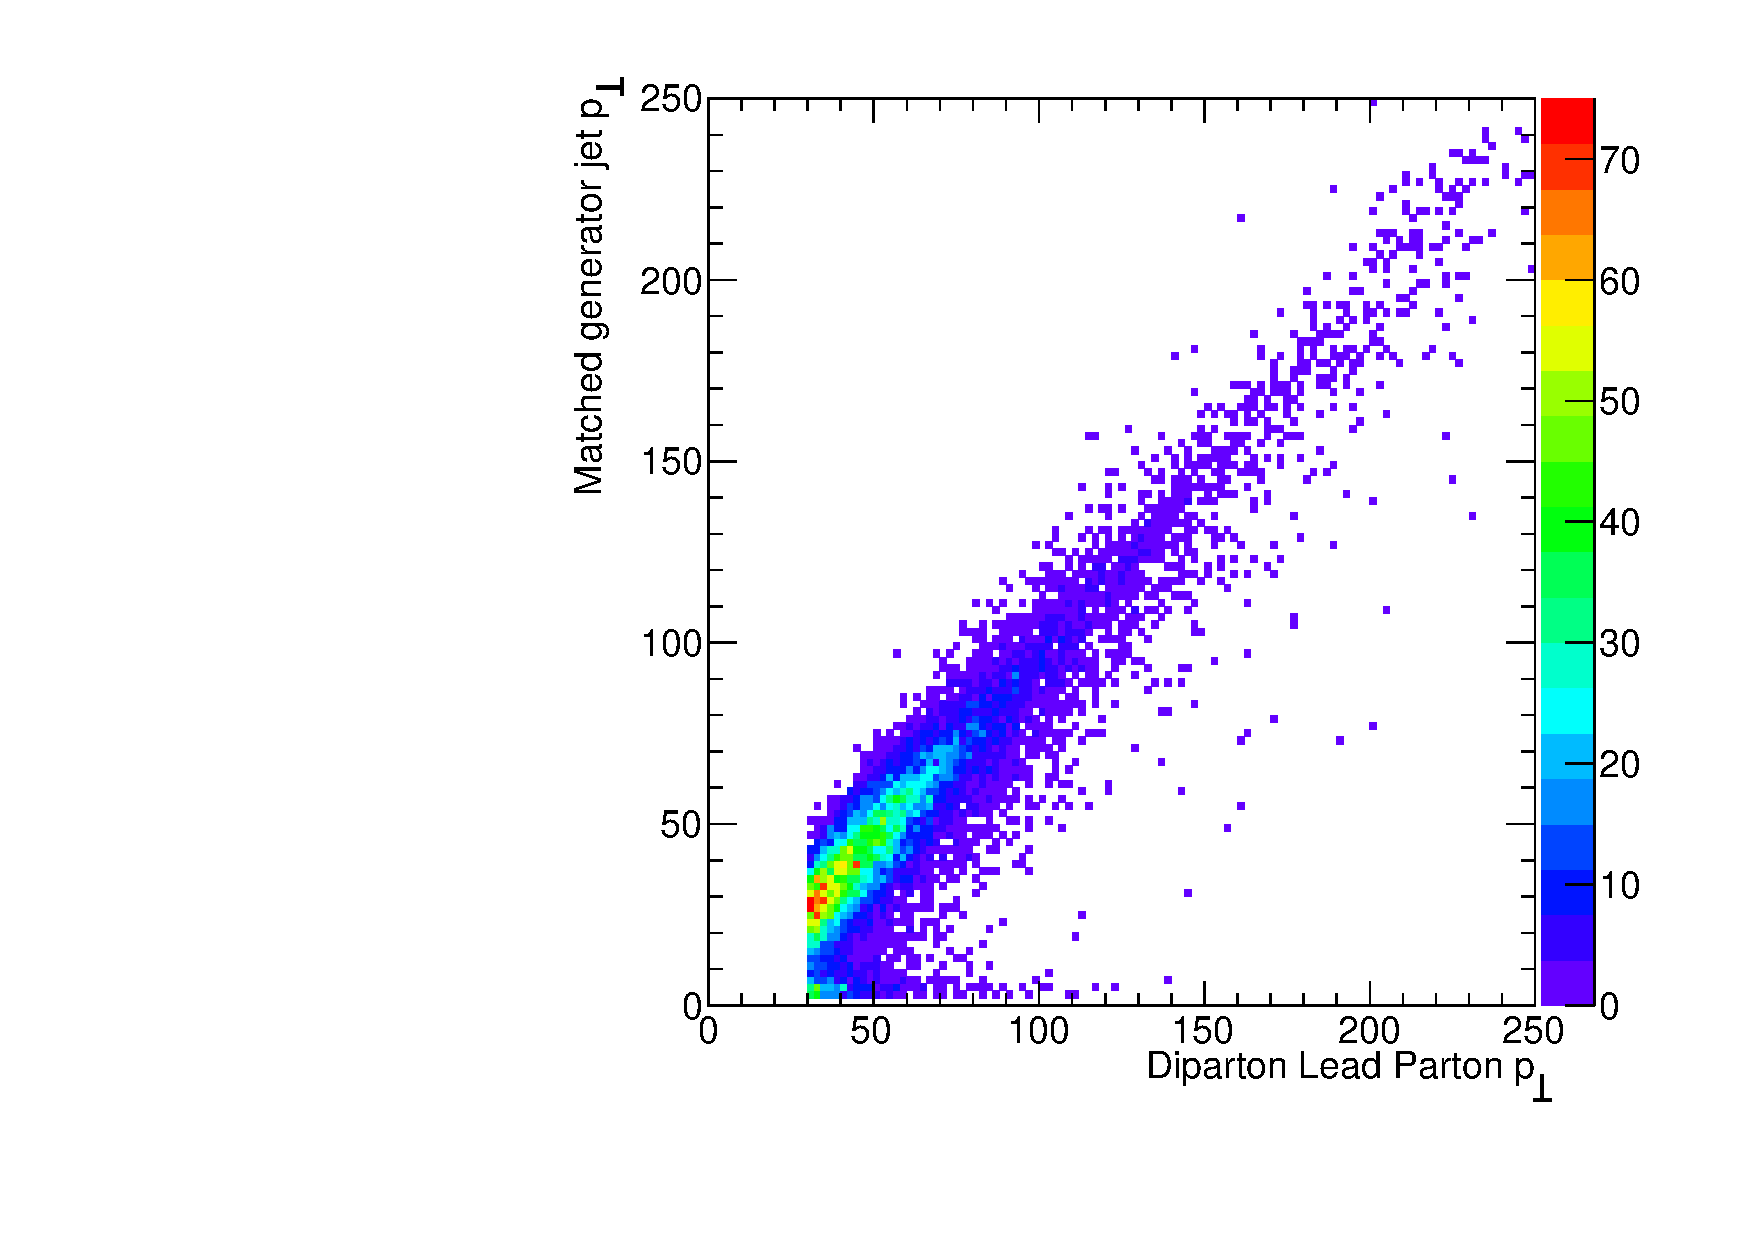
\includegraphics[width=0.45\linewidth]{Chapter07/QCDVBF/Gridpack/Images/SelDiParton_MatchedGenJet_Parton1_Pt.pdf}}\qquad
\subfloat[][]{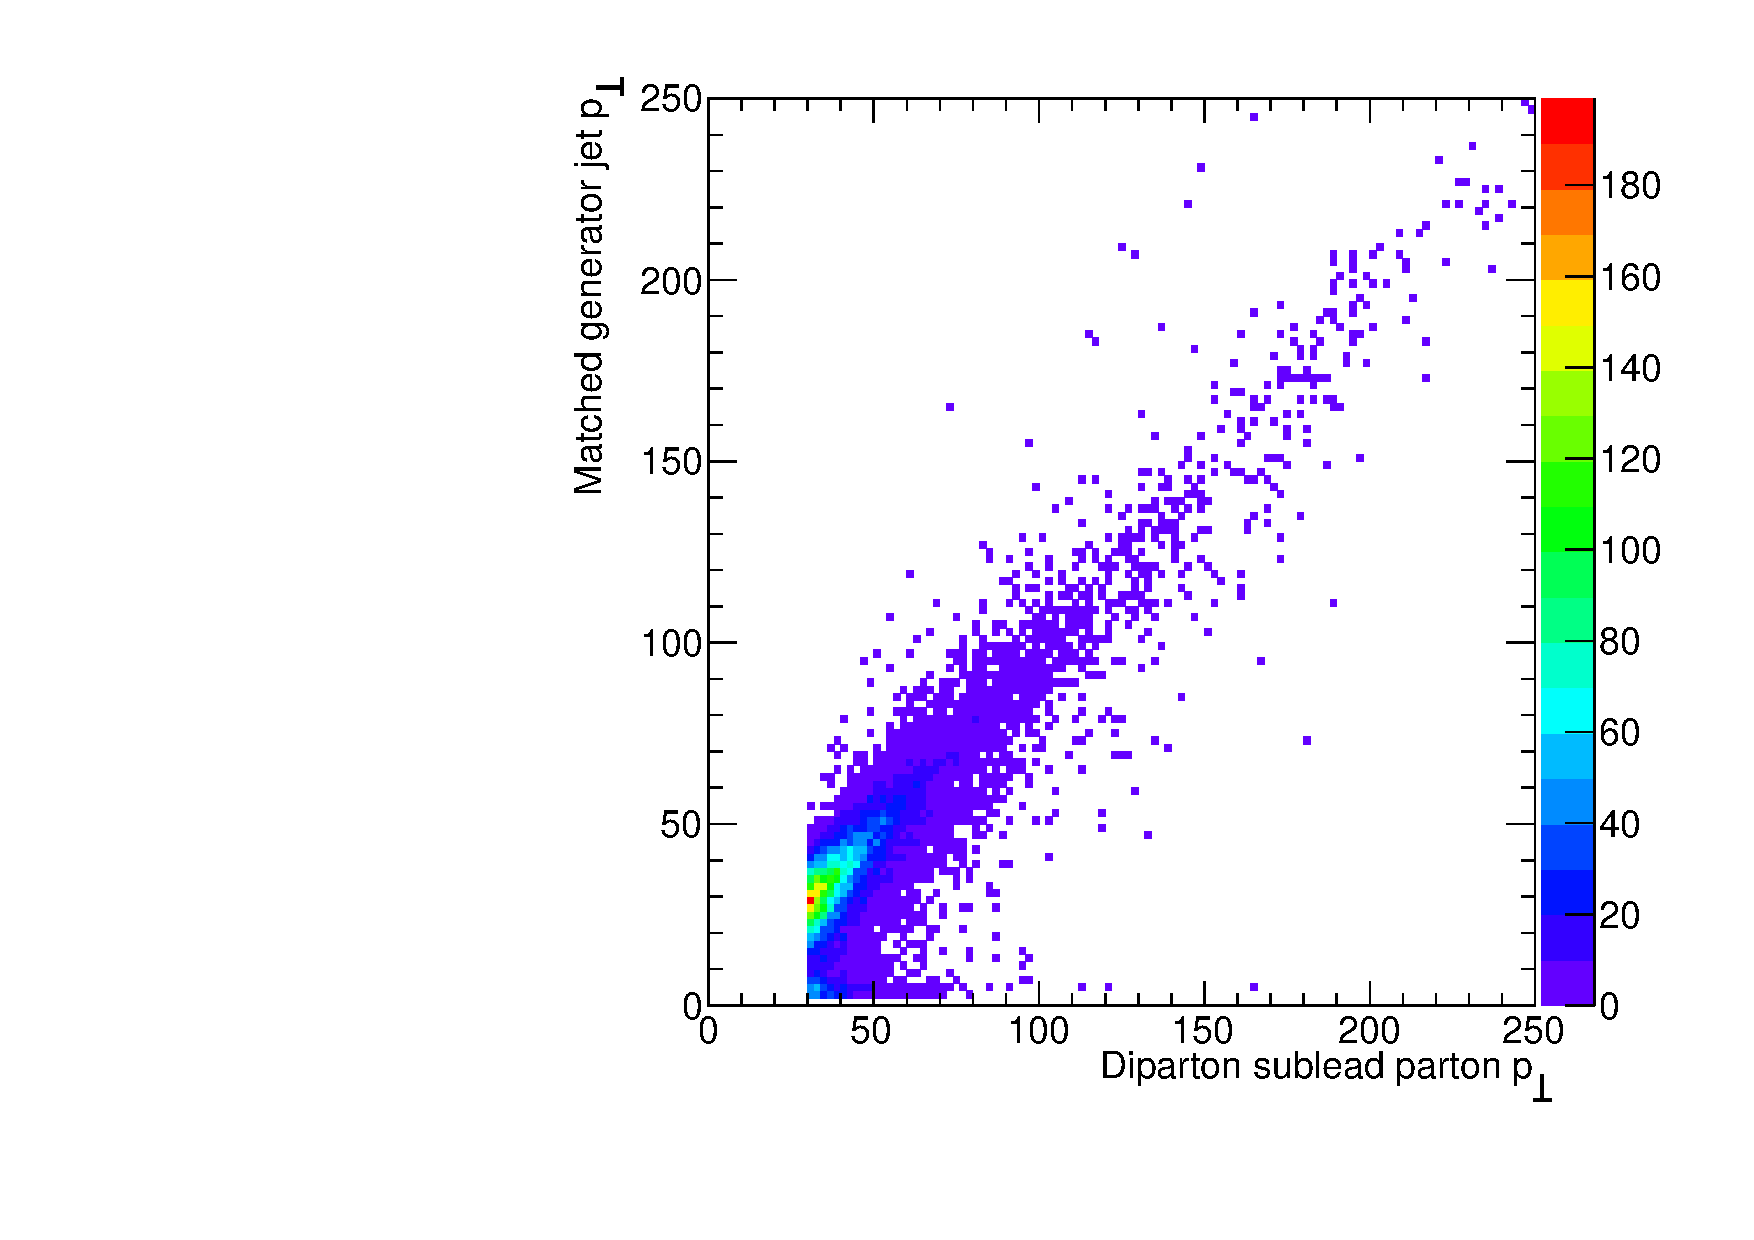
\includegraphics[width=0.45\linewidth]{Chapter07/QCDVBF/Gridpack/Images/SelDiParton_MatchedGenJet_Parton2_Pt.pdf}}\\
\caption[TODO]{TODO}
\label{FIGURE:TODO}
\end{figure}

\begin{figure}[htp]%
\centering
\subfloat[][]{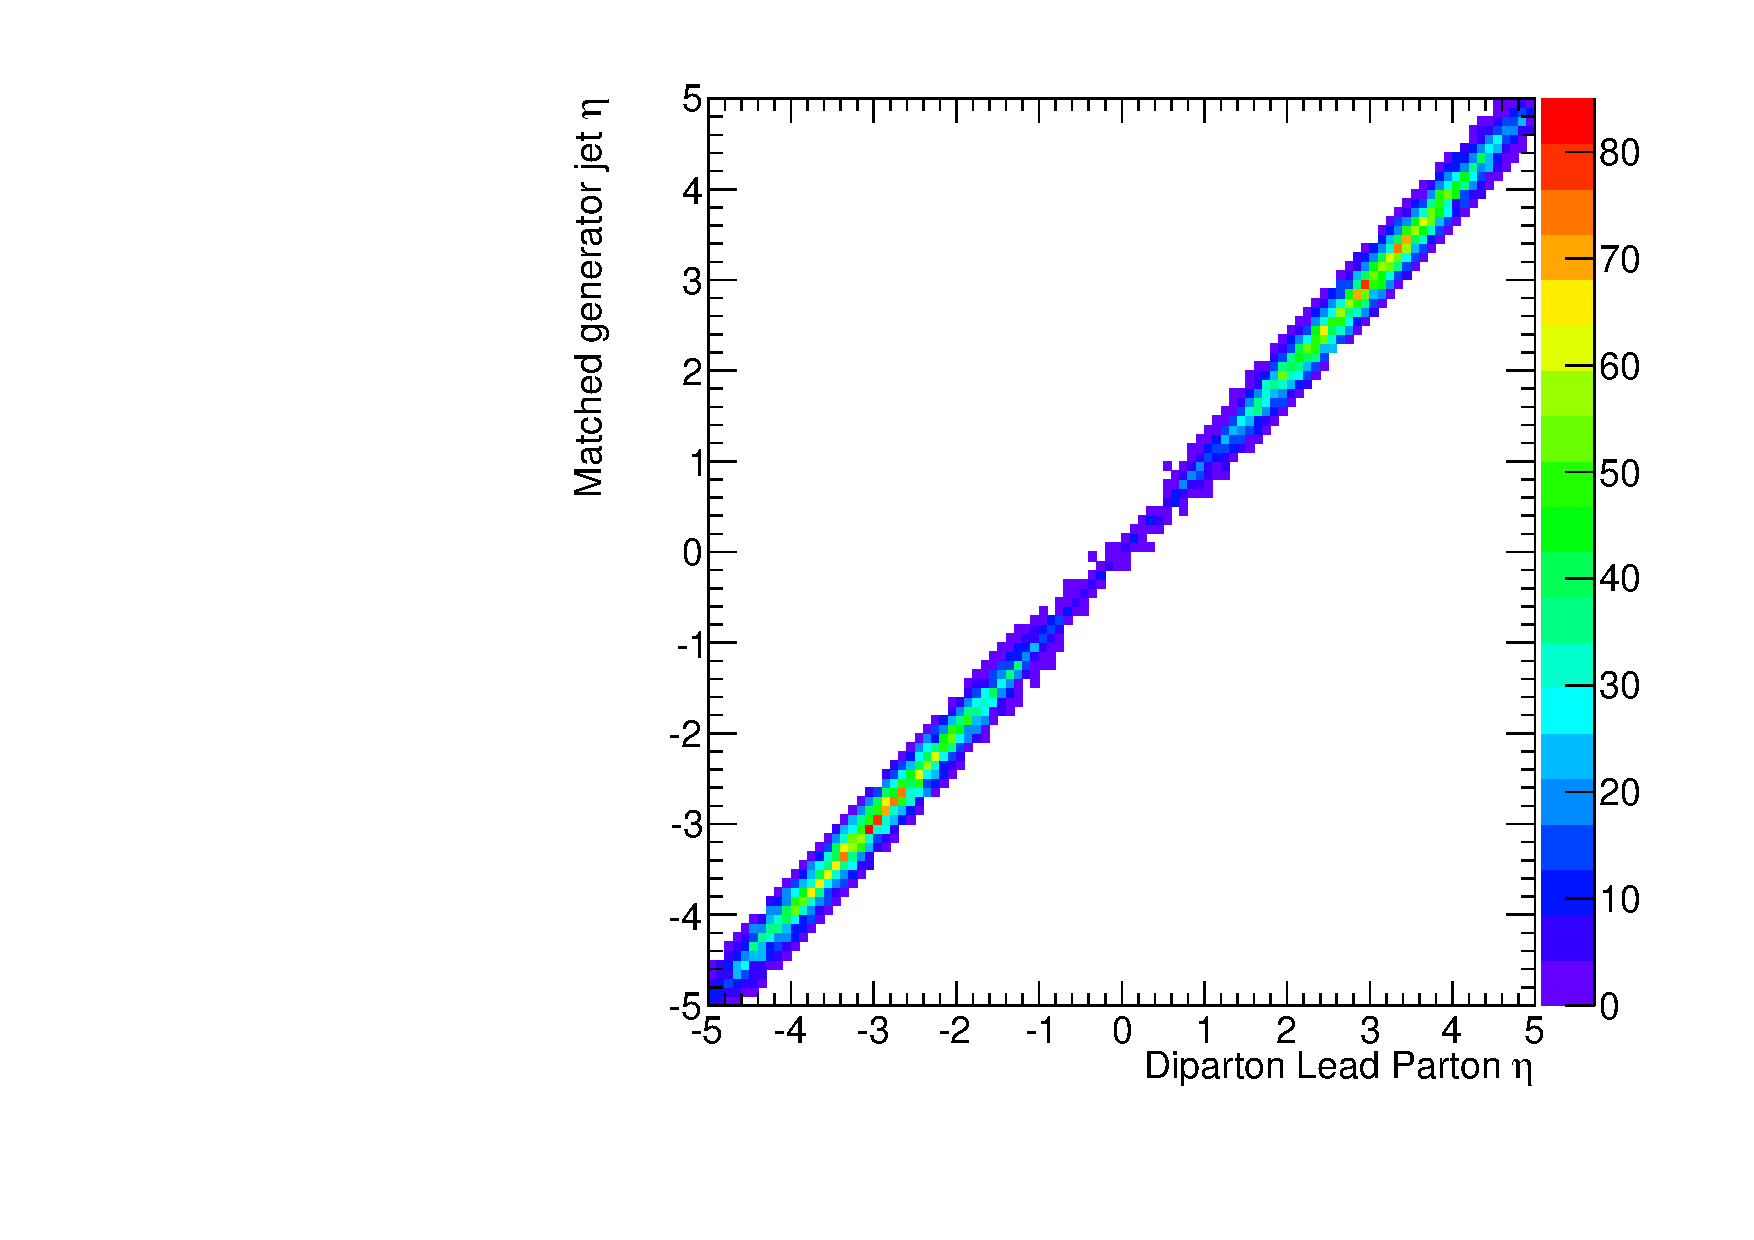
\includegraphics[width=0.45\linewidth]{Chapter07/QCDVBF/Gridpack/Images/SelDiParton_MatchedGenJet_Parton1_Eta.pdf}}\qquad
\subfloat[][]{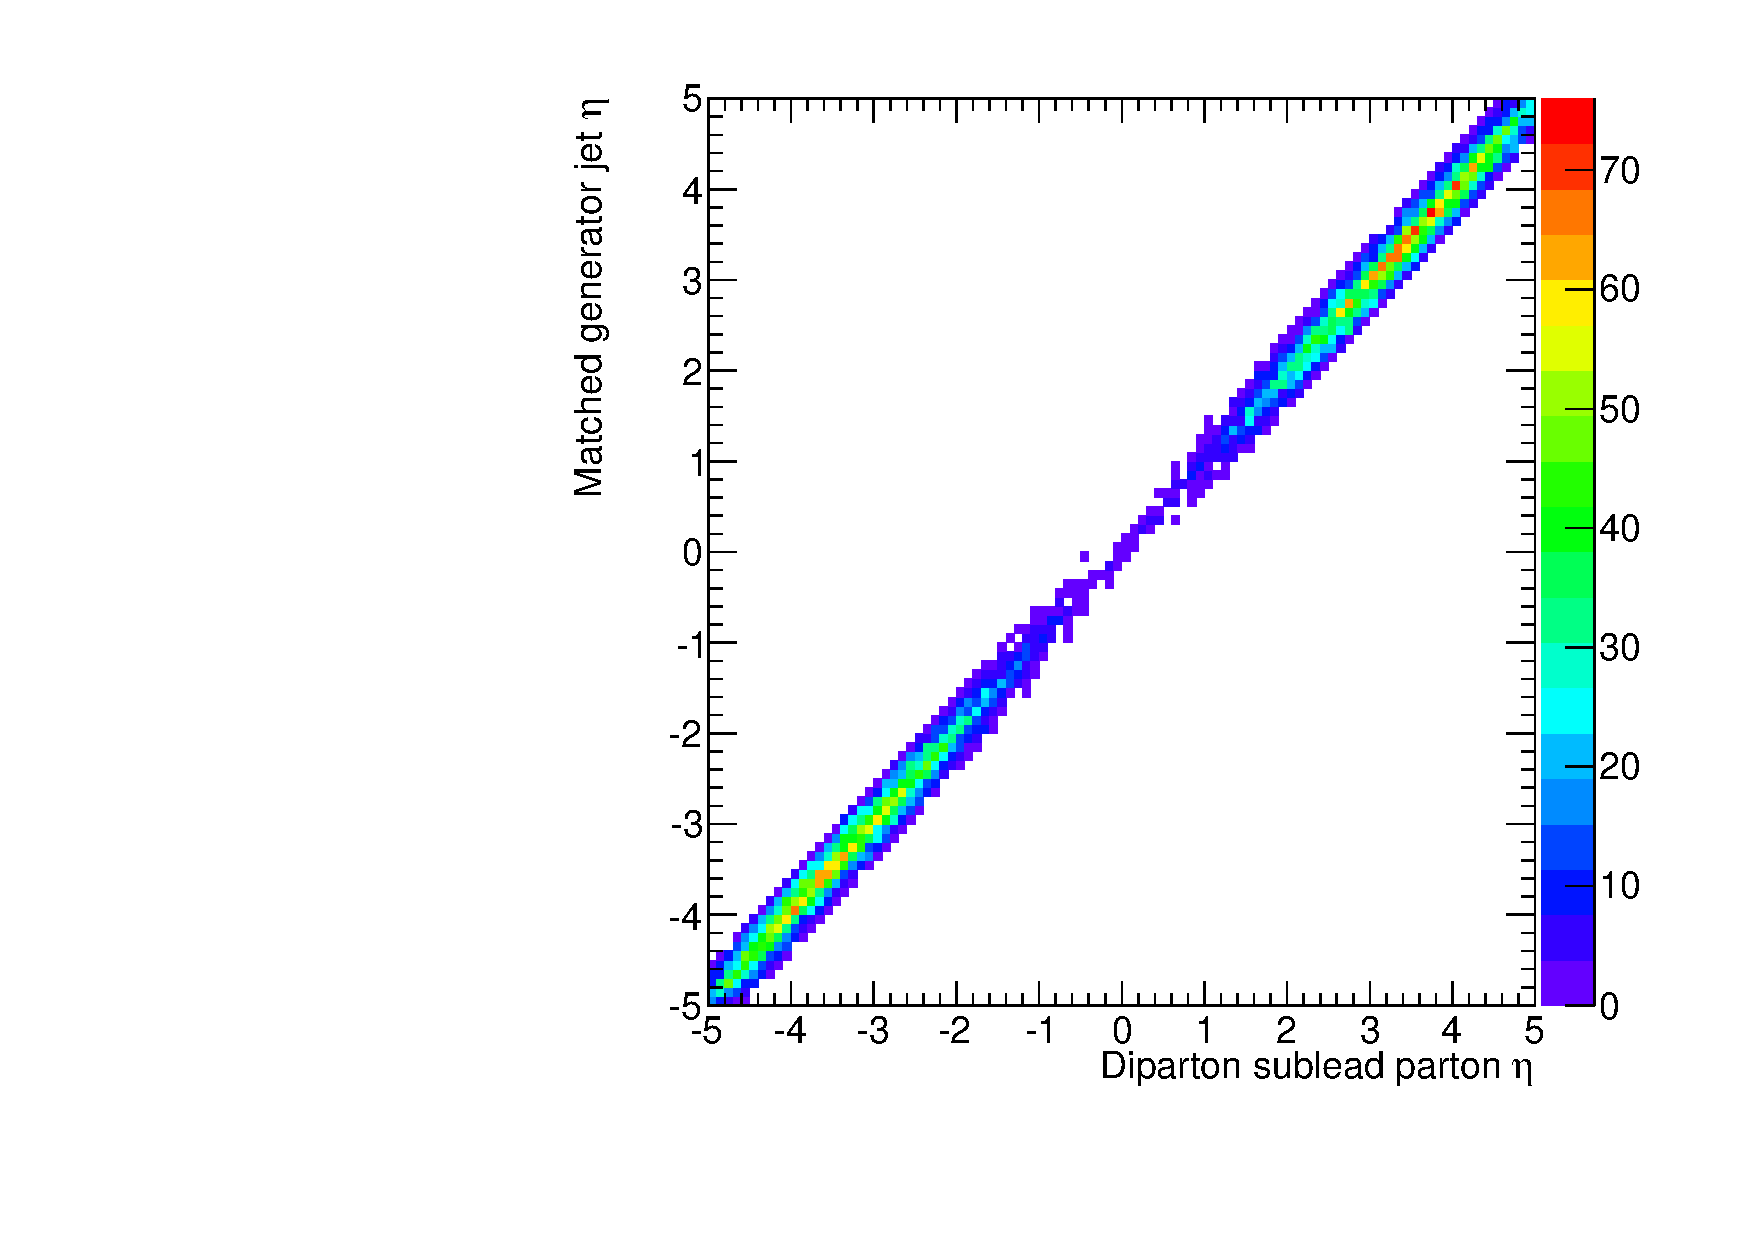
\includegraphics[width=0.45\linewidth]{Chapter07/QCDVBF/Gridpack/Images/SelDiParton_MatchedGenJet_Parton2_Eta.pdf}}\\
\caption[TODO]{TODO}
\label{FIGURE:TODO}
\end{figure}

\begin{figure}[htp]%
\centering
\subfloat[][]{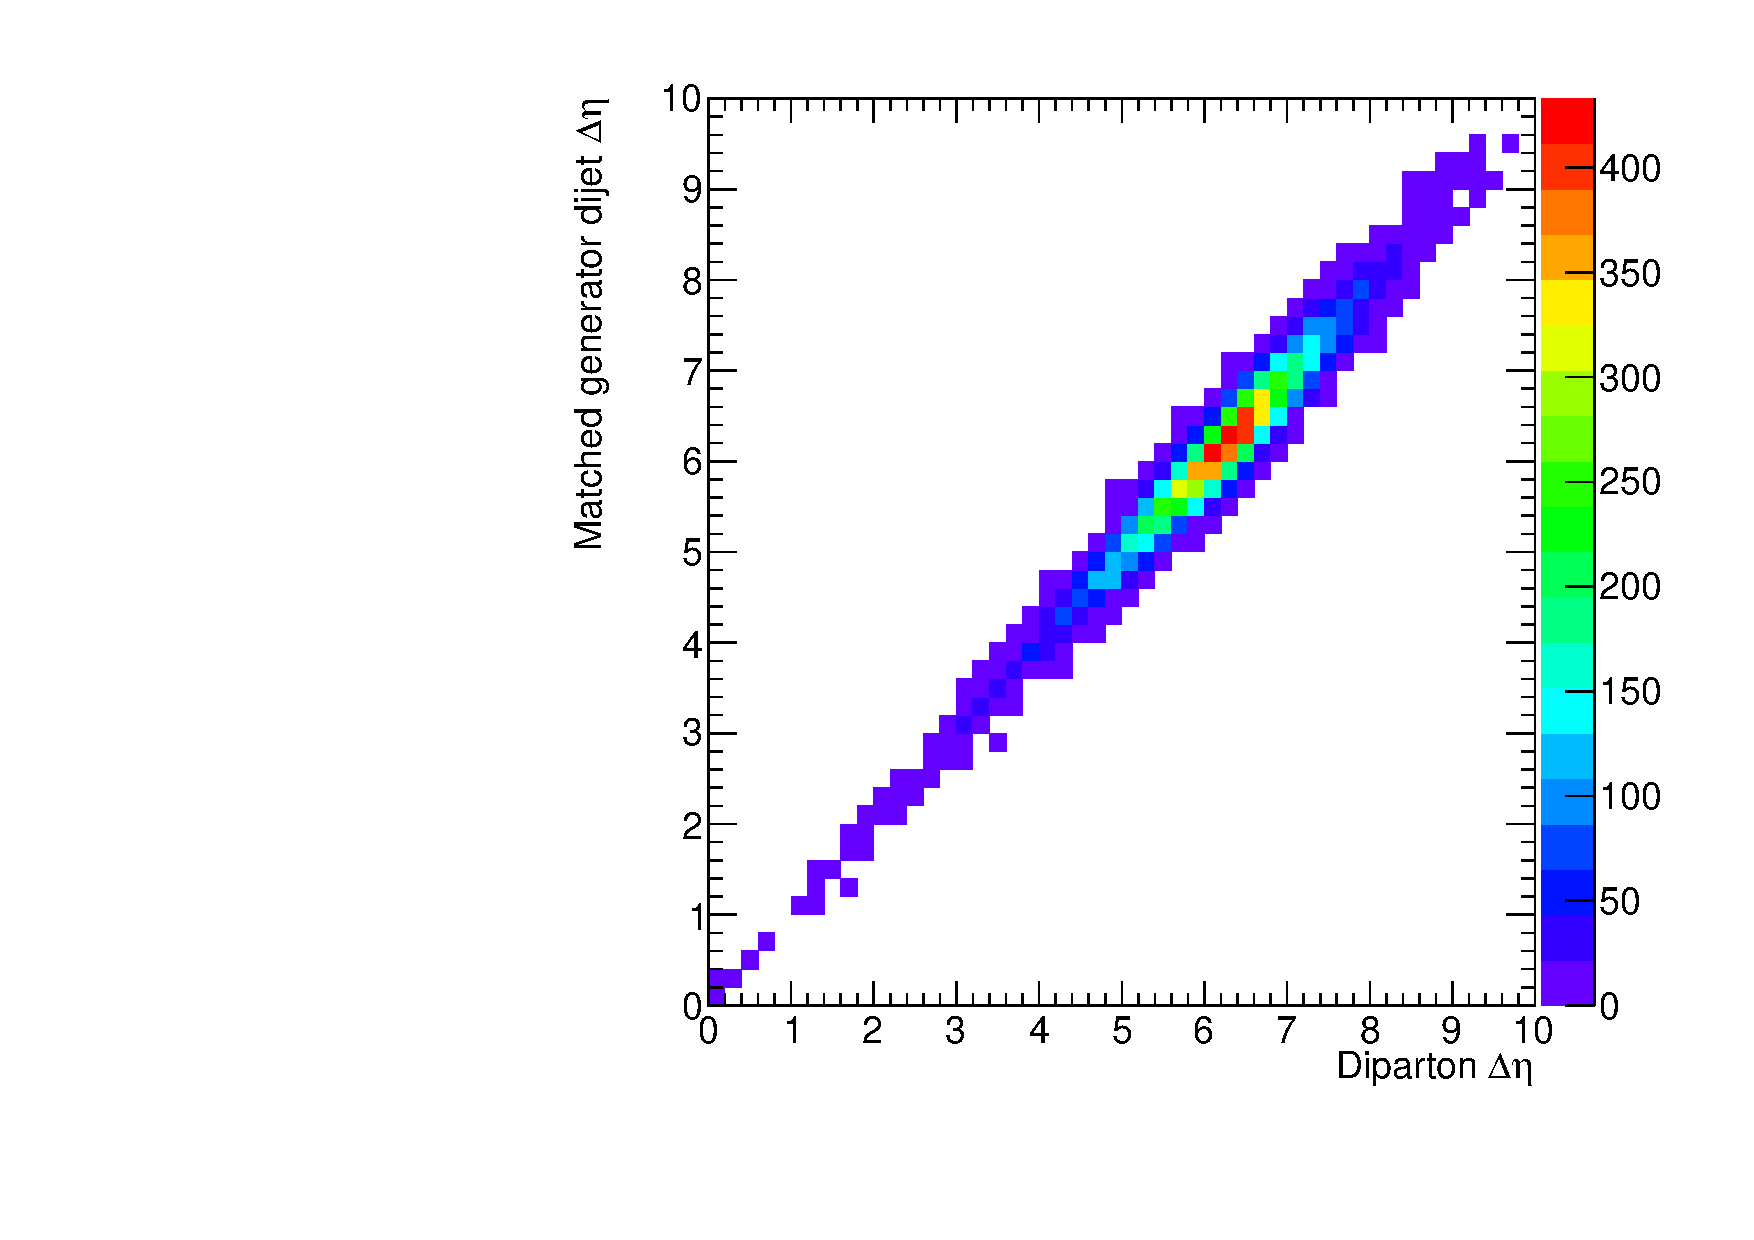
\includegraphics[width=0.45\linewidth]{Chapter07/QCDVBF/Gridpack/Images/SelDiParton_MatchedGenJet_DEta.pdf}}\qquad
\subfloat[][]{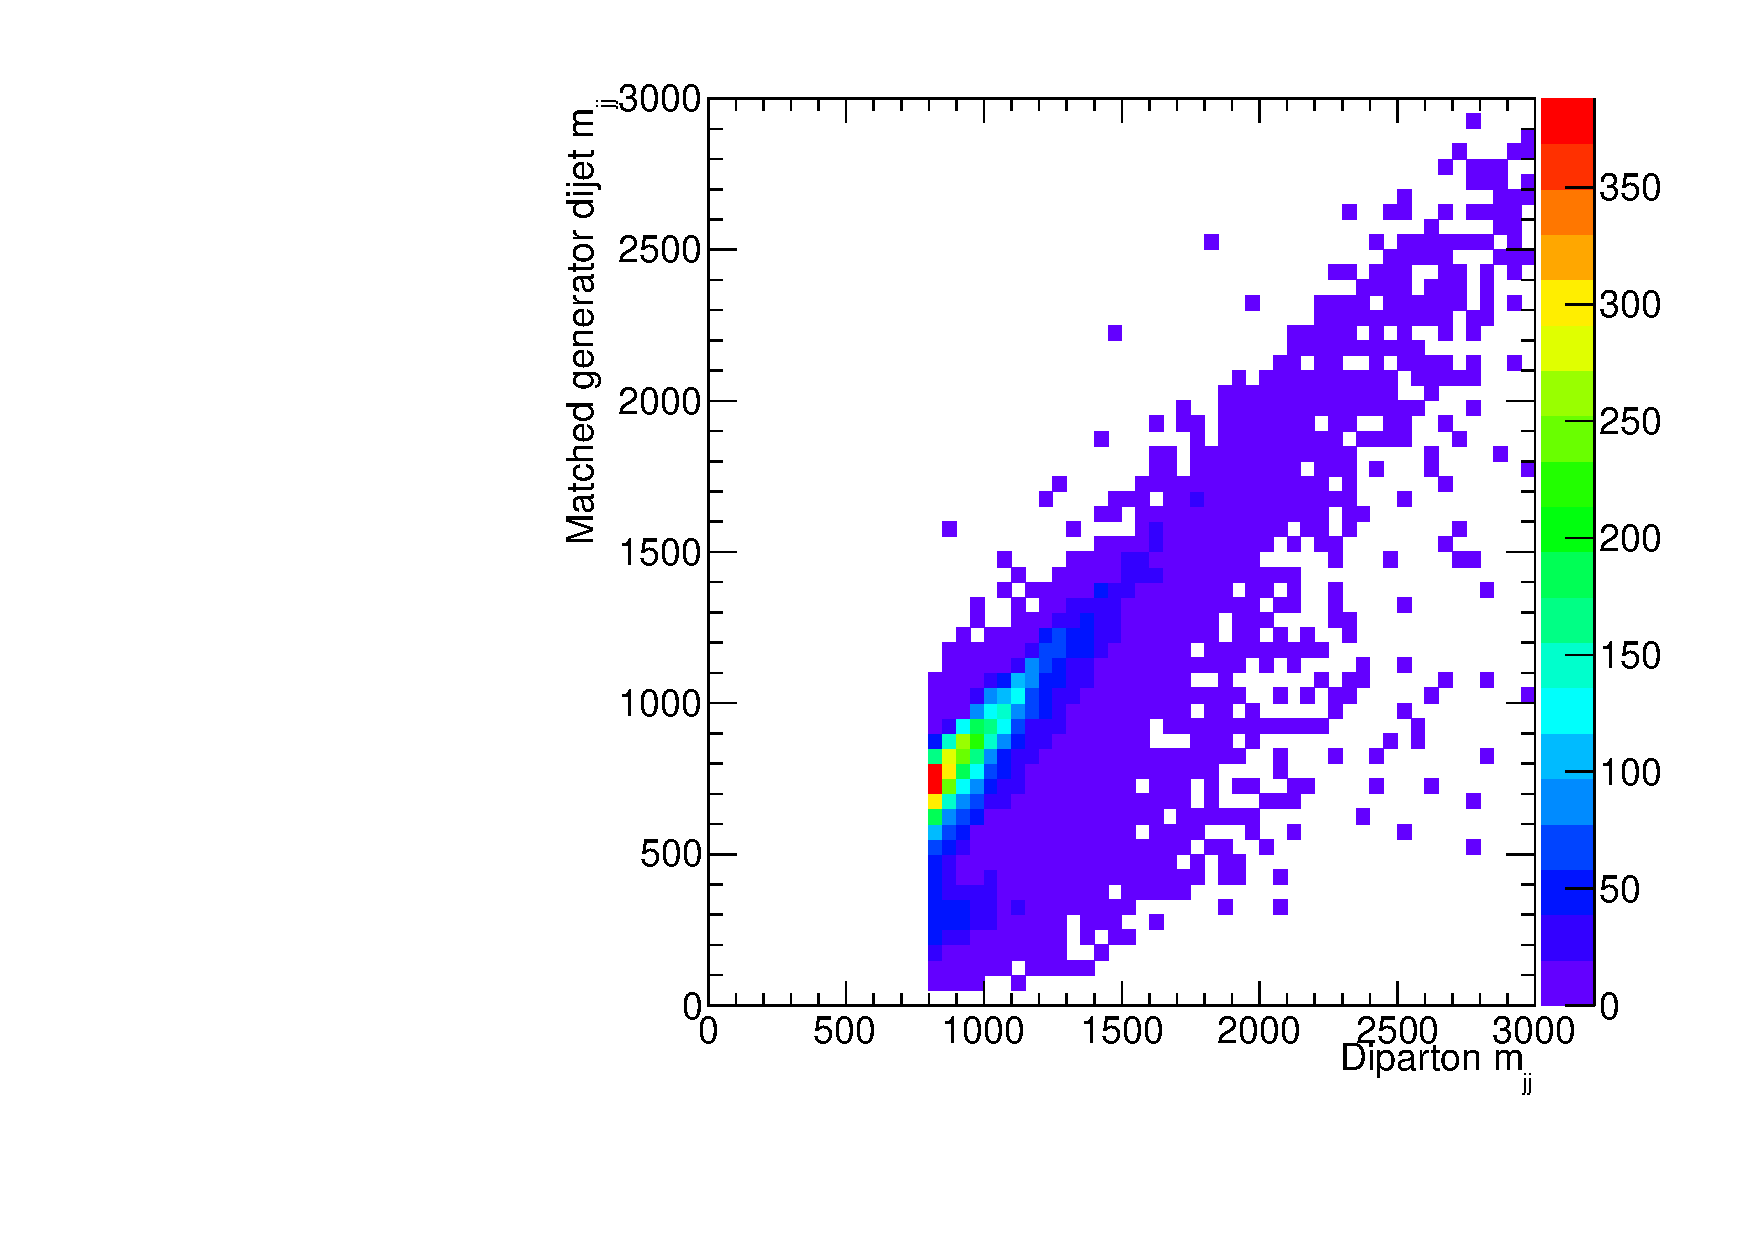
\includegraphics[width=0.45\linewidth]{Chapter07/QCDVBF/Gridpack/Images/SelDiParton_MatchedGenJet_Mjj.pdf}}\\
\caption[TODO]{TODO}
\label{FIGURE:TODO}
\end{figure}















